%! TEX root = ../thesis.tex
\section{Edit Graph}
\label{sec:collconf}

We describe the dynamics of the legislative process in terms of the conflicts between edits.
%We take a graph theoretical approach to explain our model in Section~\ref{sec:models}.
For each dossier, we construct the edit graph $ G = (V_G, E_G) $, such that each node $ v \in V_G $ is an edit and such that there is an undirected edge $ (u, v) \in E_G $ if edits $u$ and $v$ overlap.
A component of size at least~2 in $G$ is therefore a group of overlapping edits. % removed ``connected'' -> it's part of the definition of ``component'', so unnecessary
An isolated node corresponds to an edit that does not overlap with any other edit.

In Figure~\ref{fig:edit_graph}, we show the edit graphs of three regulations of EP7.
We depict each node with a green dot if the edit is accepted, and with a red cross if the edit is rejected.
The ``transportable pressure equipment'' (left), a very specific legislation, exhibits a graph with 96 nodes, among which 97\% are accepted.
The graph contains only isolated nodes, meaning that no edits overlap: all its components are size 1.
The ``European capitals of culture'' (center), which can affect some cities of member states, exhibits a graph with 58 nodes, among which 48\% are accepted.
The graph contains 16 cliques and the average component size is 1.49.
The GDPR (right), with high stakes for both businesses and consumers, exhibits a graph with 3154 nodes, among which only 9\% are accepted.
The graph contains 1298 cliques, meaning that many edits are conflicting, and has an average component size of 3.44.

\begin{figure}
  \centering
	\newcommand{\imgscale}{0.88}
	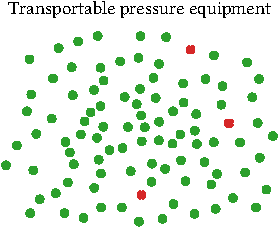
\includegraphics[scale=\imgscale]{lmp-edit-graph-tpe}\hfill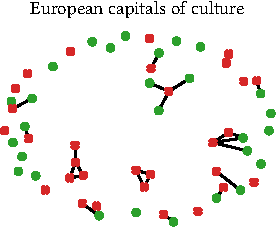
\includegraphics[scale=\imgscale]{lmp-edit-graph-ecc}\hfill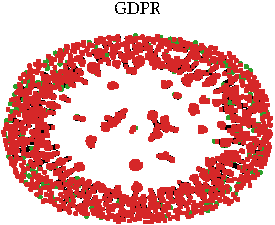
\includegraphics[scale=\imgscale]{lmp-edit-graph-gdpr}
	\caption{
		(Left) The ``transportable pressure equipment'' edit graph contains 96 edits (97\% accepted) and no conflicts.
		(Center) The ``European capitals of culture'' edit graph contains 58 edits (48\% accepted) and 16 conflicts.
		(Right) The GDPR edit graph contains 3154 edits (9\% accepted) and 1298 conflicts.
	}
	\label{fig:edit_graph}
\end{figure}

\subsection{Conflicts}

Conflicts are inherent in the ordinary legislative procedure defined in Section~\ref{sec:background}, as every proposed edit reflects a disagreement with the initial law proposal.
A first class of conflicts occur between the proposal and each edit proposed by MEPs.
These conflicts appear as components of any size in $G$.
Hence, every isolated node and every clique in $G$ are such conflicts.
We call them ``conflicts with the status quo'', as they are in disagreement with the proposal.
For example, each edit of Amendments 108 and 5 in Figure~\ref{fig:amendment} is such a conflict.
In Figure~\ref{fig:edit_graph} (left), each green node is an edit accepted over the status quo, and each red node is an edit rejected over the status quo.
Similarly, in Figure~\ref{fig:edit_graph} (center), the cliques with all red nodes are rejected over the status quo.

Another class of conflicts occur between two or more edits proposed by MEPs.
If several MEPs propose different edits on the same part of a text, they compete with each other for the acceptance of their suggestions.
In this case, the edits conflict with the status quo \textit{and} with edits proposed by other MEPs.
These conflicts appear as a clique of size at least~2 in $G$, as there is an edge between overlapping edits.
For example, in Figure~\ref{fig:amendment}, the first edit in Amendment 108 and the first edit in Amendment 5 form such a conflict.
It corresponds to a clique of size~2.
In Figure~\ref{fig:edit_graph} (left), there are no such conflicts.
As no edge links any two nodes, all conflicts are only with the status quo.
In Figure~\ref{fig:edit_graph} (center), however, the cliques with one green node and one or more red nodes are conflicts between several edits, where one edit is accepted over the others and over the status quo.

In $G$, two green nodes cannot appear at both ends of the same edge, as only one edit can be accepted among those that are conflicting.
% Hence, any clique can have at most one green node, and green nodes can only appear as an independent set on the components.
Hence, green nodes can only appear as an independent set on the components.
Two red nodes, however, can appear at both ends of the same edge, as they can both be rejected: this is the case with the first edit in Amendments 108 and 5.

Conflicts between edits can be easily projected to conflicts between MEPs, as we know the authors of each edit.
We compare the conflictive dynamics between MEPs by comparing the distribution of (i) the number of cliques and (ii) the size of cliques in the edit graph $G$ of each dossier.
The median number of cliques in EP7 is 14, which is smaller than 32 in EP8.
The median size of cliques in EP7 is 2.23, which is smaller than 2.38 in EP8.
There are therefore (i) more conflicts and (ii) conflicts of larger size in EP8, compared to EP7.
This increased heterogeneity in the clique structures of edit graph $G$ suggests that predicting the outcome of edits is more difficult for EP8.

\subsection{Collaboration}

Here, we construct the collaboration graph $ H = (V_H, E_H) $ by projecting edits onto the space of MEPs.
Each node $ v \in V_H $ is a MEP and there is a weighted edge $ (u, v) \in E_H $ if MEPs $u$ and $v$ co-sign an edit, where the weights count the collaborations.
The node-degree distribution, i.e., the distribution of number of collaborators, is well fitted by a power-law distribution whose median is 61 for EP7 and 136 for EP8.
Hence, MEPs tend to collaborate with many colleagues in general, and more so in EP8.

We quantify (i) national and (ii) political collaborations by computing the modularity \cite{newman2006modularity} in graph $H$ when defining communities by nationality or by political group.
Modularity is a measure of the strength of the community structure in a graph.
It takes values between $-1$ and $1$, with a higher positive value indicating stronger community structure.
In order to obtain comparable measurements, we merge the two right-wing populist, euroskeptic groups of EP8 to obtain 8 political groups, as in EP7\footnote{Communities of equal size are required to enable fair comparison of modularities. One right-wing populist group in EP7 split into two at the beginning of EP8.}.
We compute the modularity $ Q_n^{(l)} $ when clustering MEPs by nationality in the $l$-th legislature and $ Q_p^{(l)} $ when clustering MEPs by political group.
Computing the modularities in both legislatures, we obtain
\begin{align*}
  Q_n^{(7)} = 0.17  &>  0.05 = Q_n^{(8)}, \\
  Q_p^{(7)} = 0.22  &>  0.18 = Q_p^{(8)}.
\end{align*}
This suggests that political affinity is more important than national affinity to drive collaboration in EP8 compared to EP7.
The political science has not settled on this point: political cohesion is stronger than national cohesion in the EU Parliament in some works \cite{hix2002parliamentary,hix2008voting,mcelroy2010party}, and national cohesion is stronger than political cohesion in other works \cite{cicchi2013logic,hix2013empowerment,cencig2017voting}.
To the best of our knowledge, however, all previous work about political and national cohesion is performed using vote outcome data rather than amendment outcome, an inherently different setting.

% The voting process is simpler than the amending process explained in Section \ref{sec:background}.
% MEPs in plenary vote on reported amendments only, and not on the myriad of proposed amendments in the committees.
% Moreover, the outcome of committee votes are digitally registered only if requested by a political group or by at least 40 MEPs (they otherwise vote by show of hands).
% Vote datasets are therefore of smaller size and less rich.
